\chapter{Implementaci'on del dise'no adaptativo para la aplicaci'on m'ovil}
\label{capituloocho}
En este capitulo se explica el analisis, dise'no e implementaci'on del dise'no adaptativo para la aplicaci'on m'ovil con la proposito de cumplir el objetivo especifico \textit{Proveer un dise'no adaptativo para la aplicaci'on m'ovil} como se muestra en c'apitulo \ref{capitulouno} en la secci'on \ref{sec:oe}.

%Como se ha mencionado en el c'apitulo \ref{capitulouno} en la secci'on del objetivo especifico \ref{sec:oe}, se tiene en el presente c'apitulo como objetivo presentar el responsive de la aplicaci'on m'ovil, a trav'es de los componentes de CSS del framework ionic, que utiliza cuadrillas para proporcionar una soluci'on a la variedad  de resoluci'on de diferentes dispositivos m'oviles inteligentes y tablets.

\section{Dise'no adaptativo o responsive}
El dise'no adaptativo tiene la filosof'ia de \textit{Responsive Web Design (RWD\footnote{RWD- Dise'no web responsive})} establecida por Steven Champeon (2003) el propone solucionar los problemas de dise'no para los dispositivos u orientaci'on. Este problema se refiere al contenido para adaptar a los dispositivos creando una soluci'on 'unica.\cite{Adrian2012}. 

En este proyecto se ha utilizado para verificar la aplicaci'on m'ovil en dispositivos de diferentes tama'nos de resoluci'on de pantalla. Dicha aplicaci'on se ha desarrollado en el framework Ionic. A continuaci'on se explica el componente de Ionic para desarrollar un dise'no adaptativo.
%desarrollado una aplicaci'on m'ovil h'ibrida para el sistema operativo de android, el c'ual tiene dispositivos en diferentes tama'no de resoluci'on de pantalla. El desarrollo de la implementaci'on se ha utilizado el framework ionic.

\section{Componentes de Ionic}
El componente de Ionic el c'ual tiene un sistema cuadr'iculada con el est'andar de CSS\footnote{CSS- Hojas de estilo en cascada} y modulo flexible de la caja de layout seg'un su p'agina oficial. 
%Los dispositivos son compatibles con el framework ionic soportan la herramienta de \textit{flexbox} utiliza la herramienta grid. 
Las caracter'isticas de componentes de CSS esta representada en la figura \ref{fig:GridI}.
\begin{figure}[H]
\centering
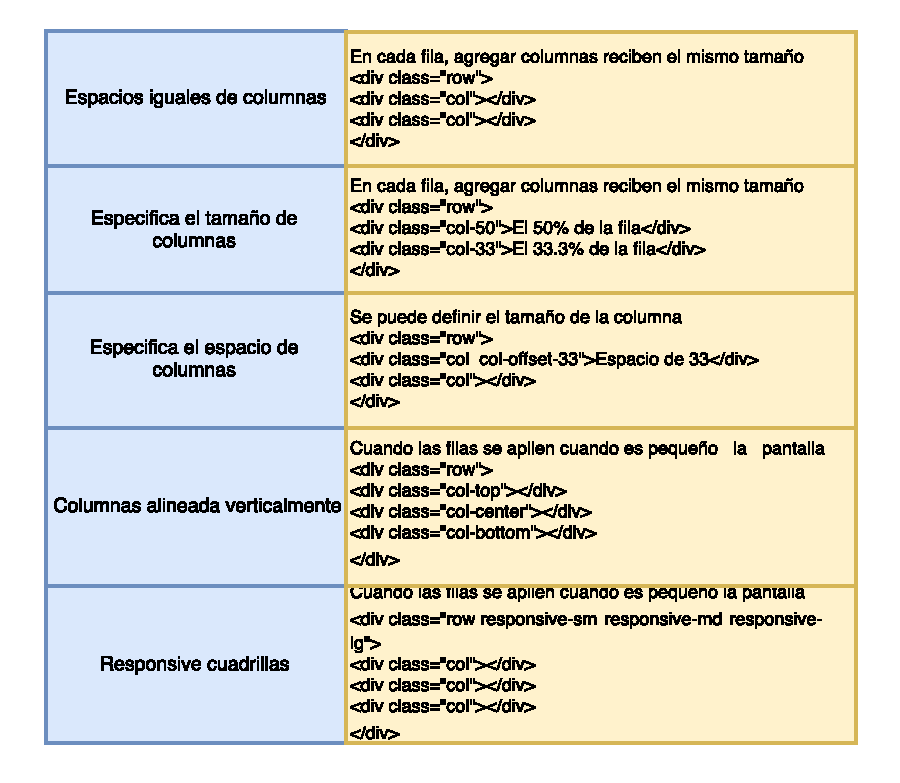
\includegraphics[width=0.6\textwidth]{gridIonic.pdf}
\captionsetup{justification=centering,margin=2cm}
\caption{Componente de CSS de ionic, Fuente: P'agina oficial}
\label{fig:GridI}
\end{figure}

\section{Implementaci'on de responsive}
Con el objetivo de implementar el responsive se ha utilizado el flexbox el c'ual se encarga de realizar los cortes de las cuadrillas en la siguiente linea de c'odigo.
\begin{verbatim}
  <div class="row responsive-sm  responsive-md">
  //El responsive-sm reduce la fila para visualizar de forma horizontal para movil
  //El responsive-md se amplia la columna de forma vertical para la tablets
  <div class="col col-33">
  \\ El col-33 define el 33% de la resolucion de la pantalla
\end{verbatim}


\section{Visualizaci'on del contenido con flexbox}
La visualizaci'on del contenido con flexbox es el resultado de la implementaci'on del responsive las diferencia se observa en la siguiente figura \ref{fig:GridI1}
%La visualizacion  se aplica el componente grid responsive de ionic, el c'ual nos ayuda en definir las filas, columnas  responsive grid donde la columna se adapta al 'area. En la siguiente figura se muestra la diferencia.
\begin{figure}[H]
\centering
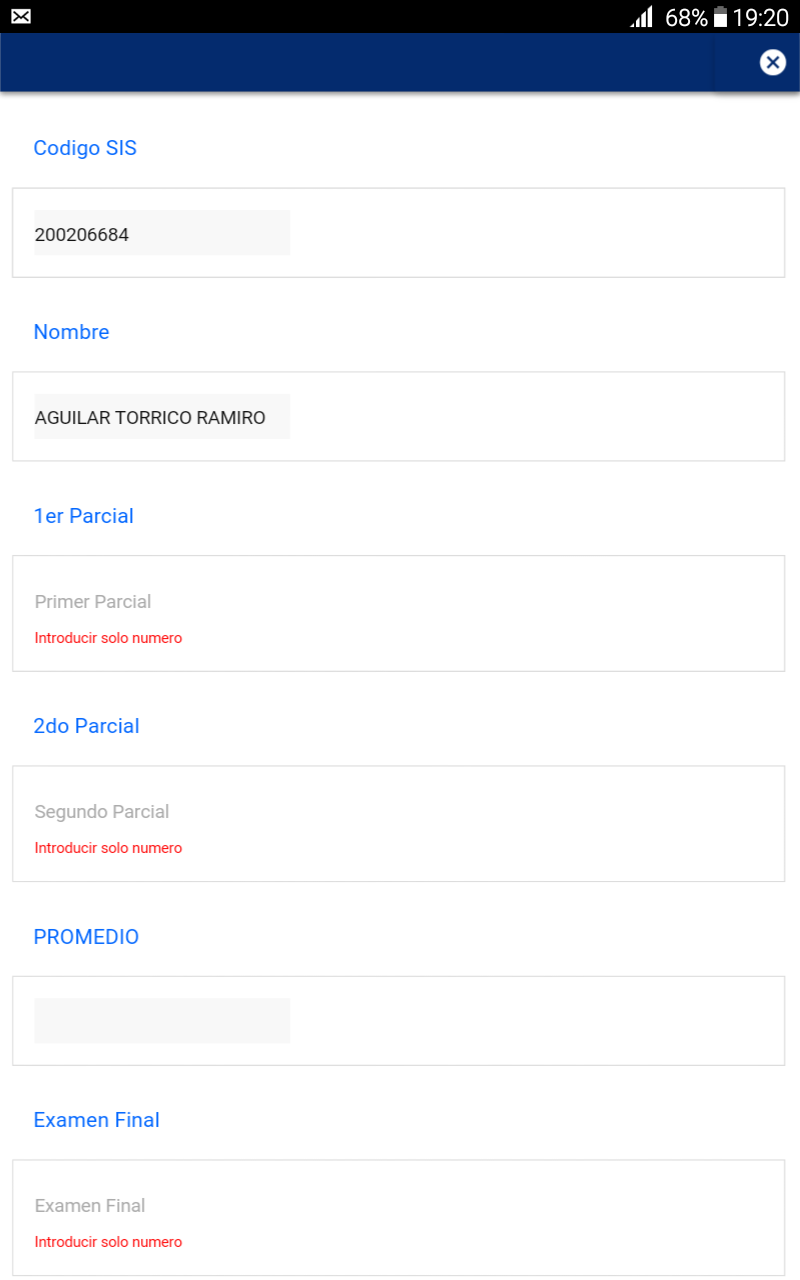
\includegraphics[width=0.2\textwidth]{gridIonic1.png}
\captionsetup{justification=centering,margin=2cm}
\caption{Visualizacion de contenido vertical en la tablet, Fuente: Elaboraci'on propia}
\label{fig:GridI1}
\end{figure}
 
En la figura \ref{fig:GridI1} se muestra la tablet con orientaci'on vertical donde las imagenes se acomodan en forma vertical y secuencial.

\begin{figure}[H]
\centering
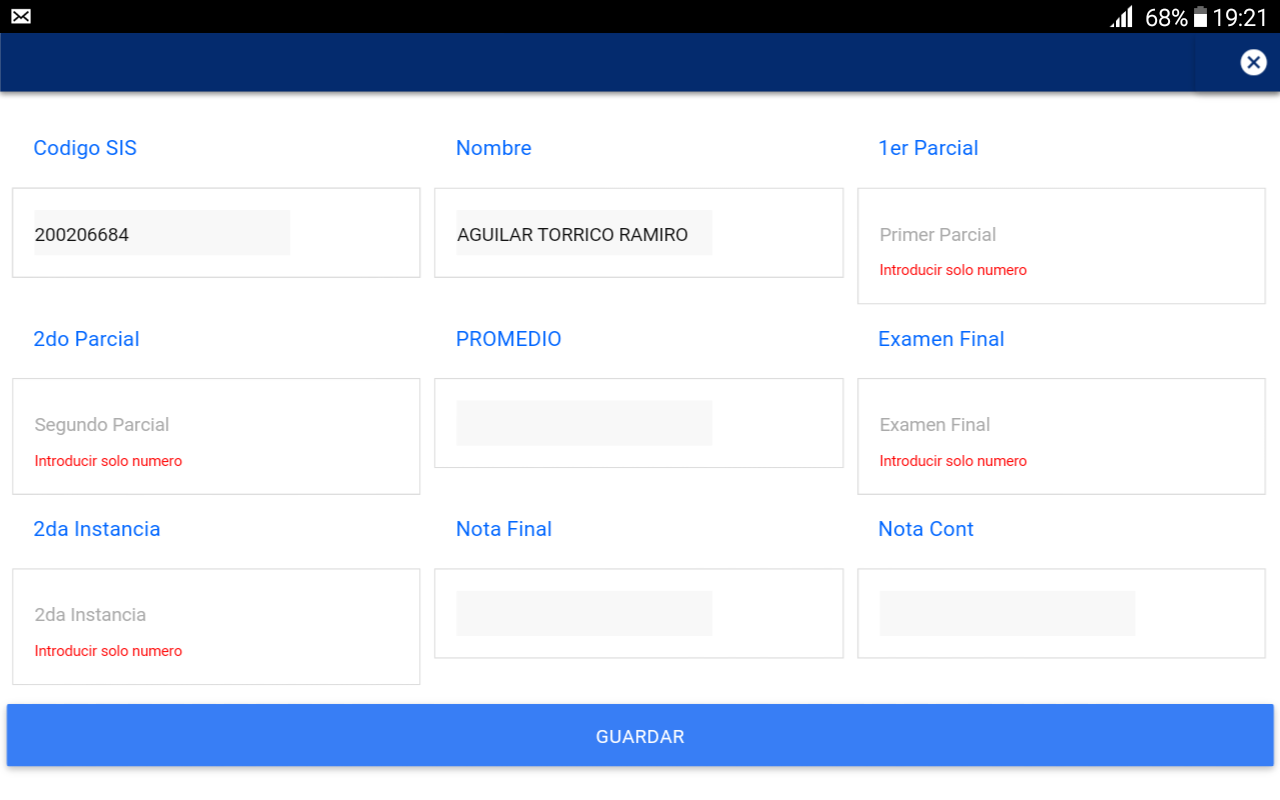
\includegraphics[width=0.6\textwidth]{gridIonic2.png}
\captionsetup{justification=centering,margin=2cm}
\caption{Visualizaci'on de contenido horizontal en la tablet, Fuente: Elaboraci'on propia}
\label{fig:GridI2} 
\end{figure}
La representaci'on de la tablet en orientaci'on horizontal y los datos se acomodan de 3 columnas debido a la resoluci'on de la pantalla como se muestra en la \ref{fig:GridI2}.